\chapter{Évolution Différentielle}

\section{Introduction}
L'Evolution Différentielle (DE) est un algorithme évolutionnaire développé par Storn et Price \cite{Storn1995} en 1995. Il est versatile et relativement simple à implémenter et utiliser, ce qui en fait un outil essentiel dans toute boite à outils d'optimisation. Comme toutes les techniques évolutionnaires, le principe de l'évolution différentielle repose sur la génération d'une population de $N_P$ solutions (ou "vecteurs") qui permettent d'évaluer une fonction objectif à des points initiaux distribués aléatoirement dans un espace de recherche borné selon l'utilisateur. Ces points sont "perturbés" dans les générations successives de la population pour essayer de trouver des solutions extrémisant la fonction objectif. L'une des caractéristiques qui font la particularité de tout algorithme évolutionnaire est l'opération utilisée pour effectuer cette perturbation. Dans le cas de l'évolution différentielle, on perturbe une solution avec la différence de deux autres vecteurs de la population, multipliée par un facteur F, c'est l'opération dite de "mutation" comme est présenté dans la figure \ref{fig:deflowchart}. Ce nouveau vecteur subit un opération de croisement avec le vecteur initial pour produire le vecteur d'essai qui est comparé avec le vecteur de même indice dans la population. Ceci est refait jusqu'à ce que tous les vecteur de la population soient comparés avec un vecteur d'essai (soit $N_P$ fois), créant la génération suivante. L'algorithme continue de créer de plus en plus de générations jusqu'à ce qu'un critère d'arrêt est satisfait. Souvent c'est un nombre de générations maximal ou une valeur de tolérance pour la variation de la fonction objectif.

\begin{figure}
  \begin{center}
    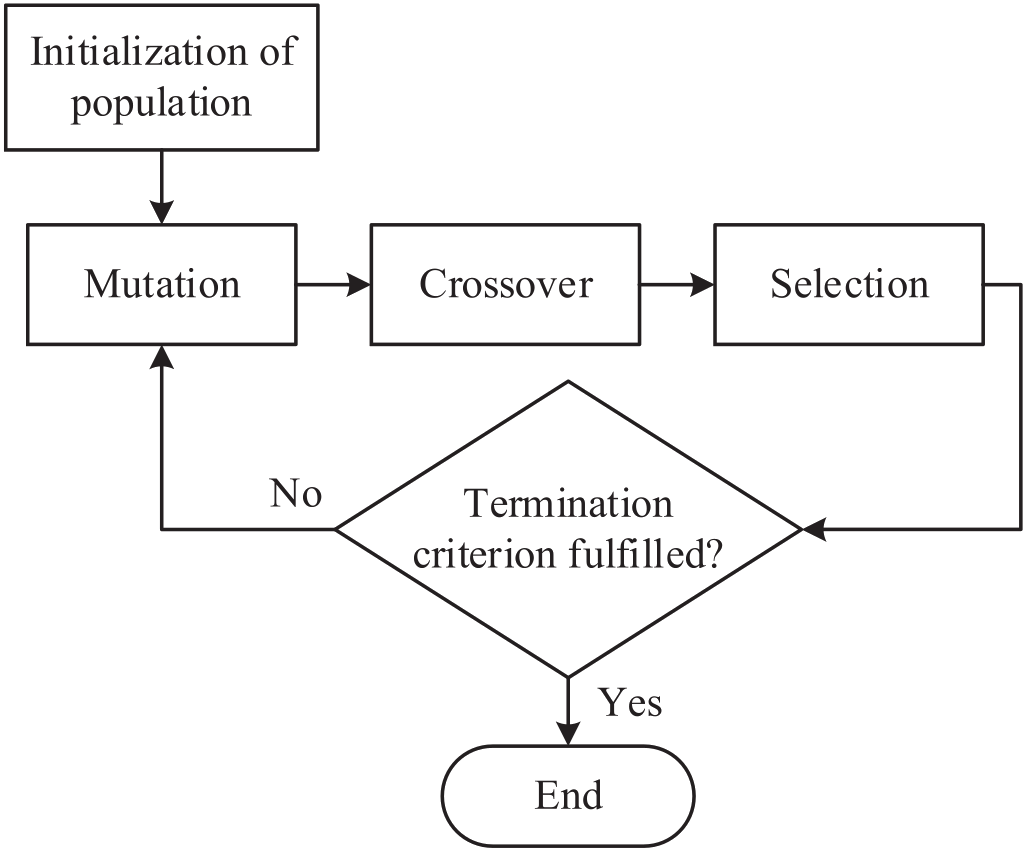
\includegraphics[width=.5\textwidth]{resources/DE.png}
    \caption{Organigramme des étapes de l'Évolution Différentielle}
    \label{fig:deflowchart}
  \end{center}
\end{figure}

\section{Description de l'algorithme}

\subsection{Initialisation}


\section{Application aux modèles simple et double diodes}

\section{Métaheuristique}

% 
